% TEMPLATE for Usenix papers, specifically to meet requirements of
%  USENIX '05
% originally a template for producing IEEE-format articles using LaTeX.
%   written by Matthew Ward, CS Department, Worcester Polytechnic Institute.
% adapted by David Beazley for his excellent SWIG paper in Proceedings,
%   Tcl 96
% turned into a smartass generic template by De Clarke, with thanks to
%   both the above pioneers
% use at your own risk.  Complaints to /dev/null.
% make it two column with no page numbering, default is 10 point

% Munged by Fred Douglis <douglis@research.att.com> 10/97 to separate
% the .sty file from the LaTeX source template, so that people can
% more easily include the .sty file into an existing document.  Also
% changed to more closely follow the style guidelines as represented
% by the Word sample file. 

% Note that since 2010, USENIX does not require endnotes. If you want
% foot of page notes, don't include the endnotes package in the 
% usepackage command, below.

% This version uses the latex2e styles, not the very ancient 2.09 stuff.
\newcommand{\cks}[1]{\emph{cks: #1}}
\newcommand{\comment}[1]{}
\hyphenation{time-stamps}
\hyphenation{i-Vo-tron-ic}

\documentclass[letterpaper,twocolumn,10pt]{article}
\usepackage{graphicx}
\usepackage{usenix,epsfig}
\usepackage{url}


\begin{document}

%don't want date printed
\date{}

%make title bold and 14 pt font (Latex default is non-bold, 16 pt)
\title{\Large \bf Automated Analysis of Election Audit Logs}

%for single author (just remove % characters)
\author{
 {\rm Patrick Baxter}\\
 Clemson University
 \and
 {\rm Anne Edmundson}\\
 Cornell University
 \and
 {\rm Keishla Ortiz}\\
University of Puerto Rico-Arecibo
 \and
 {\rm Ana Maria Quevedo}\\
Miami Dade College
 \and
 {\rm Samuel Rodr\'{i}guez}\\
University of Puerto Rico-Mayag\"uez
 \and
 {\rm Cynthia Sturton}\\
University of California-Berkeley
 \and
 {\rm David Wagner}\\
University of California-Berkeley
} % end author

\maketitle

% Use the following at camera-ready time to suppress page numbers.
% Comment it out when you first submit the paper for review.
%\thispagestyle{empty}


\subsection*{Abstract}
The voting audit logs produced by electronic voting systems contain data
that could be useful for uncovering procedural errors and election anomalies,
but they 
are currently unwieldy and difficult for election officials to use in
post-election audits. In this work, we develop new methods to analyze these
audit logs for the detection of both procedural errors and system
deficiencies. Our methods can be used to detect votes that were not included in
the final tally, machines that may have experienced hardware problems during the
election, and polling locations that exhibited long lines. We tested our analyses on
data from the South Carolina 2010 elections and were able to uncover, solely
through the analysis of audit logs, a variety of problems, including vote
miscounts. We created a public web application that applies these methods to
uploaded audit logs and generates useful feedback on any detected issues.

 

\section{Introduction}
Election officials are tasked with the difficult job of ensuring fair
  and smooth elections. It is their responsibility to ensure that ballots are
  cast, collected, and tallied properly and that every registered voter who
  comes to a polling place to vote is given the opportunity to do so. This
  requires that every polling location is staffed with well-trained poll workers
  and provisioned with enough ballots and balloting stations to accommodate all
  voters.  A number of election day events can thwart 
  even the best efforts on the part of election officials; surges of voters all
  arriving to vote at the same time, malfunctioning machines, and poll worker
  errors are a few. Information about election day events can help officials,
  and researchers who study elections, better understand
  what worked and what did not work and better prepare for the next election.

\comment{The logs this research is concerned with are produced by Direct Recording 
Electronic voting machines. A Direct Recording Electronic (DRE) voting machine is one in which
 the voter interacts directly with the terminal, typically through a touch 
screen. DREs provide a friendly interface to assist the voter with the ballot 
marking process. DRE machines can issue electronic ballots on demand; running 
out of paper ballots is no longer an issue. Additionally, audio DREs can assist
visually impaired voters.}

In the November 2010 U.S. elections, 33\% of registered voters were using Direct
Recording Electronic (DRE) voting machines~\cite{verifiedvoting-votingsystems}.
Federal standards require that electronic voting machines generate detailed
audit logs for use during post-election audits. Unfortunately, while the logs
contain large amounts of data, it is not immediately obvious what sort of useful
information can be learned from the data. Furthermore, even simple
tallies are cumbersome, time consuming, and prone to human error if done
manually. For these reasons, election officials do not regularly perform
countywide post-election analysis of the log data.

However, log data contains a trove of information that can shed light
on what takes place at the polling place on election day. For example,
election officials can use the information to learn about voting machines that
may need maintenance, or ways that poll workers and other resources may be
better allocated.

In this work, we aim to make DRE audit log analysis more useful and accessible
to election officials and other interested parties. We develop new methods to
analyze audit logs for the detection of both procedural errors and system
deficiencies. We created AuditBear, a public web application that provides our 
fully automated analyses as a free service for use by election officials or
interested third parties.  

A strength of our tool is that even in the face of missing data, we are still 
able to pull out useful information. Our research contributes to the election 
audit process in the following ways.

\begin{itemize}
\item We introduce methods for identifying, solely from publicly available audit
  logs, potential errors in the software, hardware, and system configuration of
  DREs.
\item We introduce methods for identifying instances of human error by poll
  workers. Furthermore, we differentiate between random
  errors and patterns of error that suggest shortcomings in the training
  election workers receive.
\item We introduce a new method for conducting a statistical analysis of voter
  flow. This allows for improved resource allocation in future elections.
\item We conduct a case study using our methods and identify instances of poor
  worker training, long voting lines, and missing votes during the 2010 South
  Carolina election.
\item Using our experience with the case study, we suggest new content that, if
  included in election log files, would allow for additional useful analysis.
\end{itemize}

We implement these methods for the ES\&S 
iVotronic DRE; the 2010 South Carolina data was already publicly available 
through a previous Freedom of Information Act request and the iVotronic was 
used in that election. The iVotronic system is a standalone, portable, 
touchscreen system that records vote totals, ballot images and an event log 
on internal flash memory. The iVotronic voting machine is one of the most 
widely deployed DREs in the U.S. In 2010, 422 jurisdictions tallying more 
than 22 million registered voters used this system~\cite{VerVot2010}. In 
addition, the types of analyses we identify and our algorithms for analysis 
are applicable to other DRE voting systems that produce the necessary audit 
logs. \comment{We show how the audit log data can be used to detect votes that may 
have been left out of the official results, incorrect procedures being 
followed at the precincts, precincts that had to stay open late, and even 
errors in the collection of the audit data itself. These reports can help 
election officials, researchers, and fair election advocacy groups better
understand the events that took place during and after an election. }

\comment{
Many studies have shown the various security weaknesses of DRE machines
\cite{appel-evtwote09, butler-evt08, calandrino-toptobottom}. 
While many states are moving away from this method of voting for these reasons, 
DREs are still in widespread use and our tool provides easy-to-apply techniques 
that make results and future elections more reliable.  The iVotronic may be
susceptible to many security exploits, and our tool does not aim to detect 
or prevent these; rather than making DREs more secure, our tool aims to make them 
more reliable. While it is crucial to discover machines that experience malicious 
tampering, finding a number of uncounted votes or learning where voters may be
discouraged from voting by long lines is important too. In this work we 
assume that DRE audit logs are complete, accurate, trustworthy,
and free of accidental or malicious tampering. Detecting and preventing audit
log tampering is outside the scope of this work. 
}
In this work we assume that DRE audit logs
are complete, accurate, trustworthy, and free of accidental or malicious
tampering
Many studies have examined the various security weaknesses of DRE machines. DREs
have been found to be susceptible to poor software
engineering practices leading directly to exploitable
vulnerabilities~\cite{kohno2008, butler-evt08}, insider attacks~\cite{appel-evtwote09}, viruses that spread
between voting machines and the election management system
server~\cite{calandrino-toptobottom, Feldman07},  and
return-oriented programming exploits~\cite{Checkoway2009}. In all these cases, the demonstrated
payload is usually a vote-stealing or vote-altering attack and often the
associated logs and counters are modified to remove any traces of the attack. 
The iVotronic may be susceptible to many security exploits, and our tool does
not aim to detect or prevent these; detecting and preventing audit log tampering is outside the scope of
this work. Rather than making DREs more secure, our tool aims to make them  
more reliable. While it is crucial to discover machines that experience malicious 
tampering, finding a number of uncounted votes or learning where voters may be
discouraged from voting by long lines is important too. While many states are
moving away from the use of DREs precisely because of their security failings,
DREs are still in widespread use and our tool provides easy-to-apply techniques
that make results and future elections more reliable.

\section{Background}
\subsection{Introduction to the iVotronic DRE}
A brief description of the iVotronic's functionality and its main system
components follows.  

\begin{description}
\item{Voting terminal.} The voting terminal is a stand-alone touchscreen voting
  unit. It is equipped with an internal battery, which keeps the unit operational 
  in the event of a power failure.  The terminal 
  features three internal flash memories, which store the votes and terminal audit 
  data during the voting process. Three memories are used for redundancy as the 
  three store the same data.  A removable compact flash card (CF) is installed in 
  the back of the terminal prior to deployment to the precinct; this is 
  used to store audit data and ballot images (cast vote records). Typically, 
  each polling location is assigned several iVotronic machines as well as one audio 
  (ADA) terminal .
\item{Personalized Electronic Ballot (PEB).} The PEB is a proprietary cartridge
  required to operate the iVotronic terminal. The voting terminal is 
  delivered to the precinct with no ballot style information; that is later supplied 
  by the PEB. The PEBs are programmed at election central with the ballot data
  for each voting location. At the opening of the polls, poll workers 
  download ballot style information from the PEB's internal flash memory to the terminal.  When the PEB is 
  placed in the 
  machine, the terminal and the PEB can communicate through an infrared port.  
  Typically, counties deploy two types of PEBs to the precinct: a) a Master PEB
  and b) an Activator PEB. They are interchangeable, but poll workers are trained 
  to keep them separate and use them for different purposes.
\begin{itemize}
\item{Master PEB.} Poll workers use the master PEB to open and close all
  terminals on election day. The same master PEB should be used to open all 
  terminals in the polling location.  In the same fashion, the master PEB should
  be used to close all terminals in the polling location at the end of the voting
  day.  When a terminal is closed, it uploads its vote totals onto the PEB 
  inserted into it. The Master PEB accumulates the precinct totals so that they can 
  later be transported to the tabulation center where the vote totals are uploaded 
  (through PEB readers) and included in the official tally.
\item{Activator PEBs.} Activator PEBs are used by poll workers to activate ballots
  for voters. Each voter's session with the voting terminal starts with a poll
  worker inserting an Activator PEB into the terminal. Election officials provide 
  each precinct with multiple Activator PEBs. \comment{Internally, all PEBs at the precinct 
  are identical. The only difference between the two types is the color 
  of the rubber band on their exterior. Thus, a Master PEB can be used to activate 
  a voter's ballot and an Activator PEB can be used to open and close terminals;
  though,  
  as a matter of procedure and training, they should not be used this way. Poll workers are trained to put the Master PEB, CF 
  cards and precinct's total tapes in a designated bag that is transported to Election Central 
  after polls close.  Activator PEBs used to close terminals may be left behind and their 
  vote data not added to the certified count. Thus, if an Activator 
  PEB is used to close terminals, the precinct vote totals may be only partially uploaded to the 
  aggregated totals on election night.}
\end{itemize}

Internally, all PEBs at the precinct are identical. The only
difference between them is the color of the rubber band on their
exterior. Thus, a Master PEB can be used to activate a voter's ballot
and an Activator PEB can be used to open and close terminals; though,
as a matter of procedure and training, they should not be used this
way. Poll workers are trained so that they put each precinct's Master
PEB, CF cards and totals tapes in a designated bag that is
transported to Election Central after polls close; Activator PEBs
may be left behind. Thus, if an Activator PEB is used to close terminals, its
vote data may not be uploaded to the aggregated totals on
election night.

\item{Removable Compact Flash (CF) card.} The CF cards are programmed at Election
  Central and installed in the back of the voting terminal prior to deployment
  at the polling location. The CF cards contain graphic (bitmap) files read by 
  the voting terminal during the voting process. The audio files required for the 
  ADA terminals are also stored in the CF cards. The CF cards are also used as an 
  external memory device as the terminal's event log and ballot images are written 
  to the CF card when the terminal is closed for voting. Once the polls close, the 
  CF cards are removed from the back of the terminal and delivered to election 
  headquarters on election night. The CF cards are uploaded to the election management 
  system during the canvassing process. Election officials generate the election's 
  ballot image and event log databases from each precinct's set of CF cards.  For the 
  remainder of this paper, any reference to the iVotronic logs will refer to the 
  aggregated data from all precincts in a single county.
\end{description}

\comment{Include a paragraph about how the data is aggregated.}

\subsection{iVotronic Audit Data}
The ES\&S voting solution produces many log files, but in our analysis we focus
on three: the event log (EL152.lst), the ballot image file (EL155.lst), and the
system log (EL68a.lst). Other files produced by the iVotronic are the Unofficial Precinct Report-Group
Details (EL30a.lst), the Official Precinct Report (EL30.lst), the Unofficial Summary 
Report-Group Details (EL45a.lst), the Official Summary Report (EL45.lst), and the 
Manual Changes Log Listing (EL68.lst). We did not use these for two primary reasons: 
first, unofficial data detracts from the validity of our analyses; second, these 
logs were not available for the majority of counties. There is limited documentation 
about the iVotronic logs; therefore there may be additional files 
that have not been released to the public.

The event log (EL152.lst) contains audit
log entries from each iVotronic terminal used in the election. The log records,
in chronological order, all events that occurred on that machine during the
election. It typically begins at election headquarters, before the election, 
with a \textquotedblleft clear and test\textquotedblright \hspace{1 mm} of the 
terminal to delete previous election data from the terminal's memory.  It also 
records all election day events, including polls open and polls closing and 
the number of ballots cast. Each event log entry includes the iVotronic's 
terminal serial number, the PEB's serial number, the date and time, the event 
that occurred and a description of the event.

The ballot image file (EL155.lst) 
contains all ballot images saved by the iVotronic terminals during the voting
process. An ES\&S ballot image is a bit of a misnomer and might more rightfully
be called a cast vote record: it is a list of all choices made for each vote 
cast; it is not a scanned or photographic image. However, we stick with the
ES\&S terminology and refer to each cast vote record as a ballot image. The ballot images are 
segregated by precinct and terminal where the votes were cast. The ballots are 
saved in a random order to protect the privacy of the voter.

The system log listing file (EL68a.lst) chronologically tracks activity in the
election reporting database at the election headquarters. Its entries reflect 
the commands executed by the operators during pre-election testing, election 
night reporting, post-election testing and canvassing.  It also contains the totals
accumulated in the various precincts during election night reporting, as well as
any warnings or errors reported by the software during the tabulation
process. The system log also tracks the uploading of PEBs and CF cards to the
election-reporting database. Manual adjustment of precinct totals are also recorded 
in the system log file.

\subsection{Voter Privacy}
Our tool depends on the audit logs being publically available. It is important
that neither the logs themselves, nor our analyses endanger voter privacy. 

None of the logs we use in our analyses contain personally identifiable
information. The event log contains the times and machines on which votes  
were cast, but contains no voter information and no form of a ballot image. It
simply  
states that a vote was cast on machine X at time Y. The ballot images file is a 
record of all cast ballots.  Each ballot image 
depicts the choices a voter made, which machine they used, and which precinct they 
voted in. In order to protect voter privacy, the system records the ballot images 
in a random order. As long as no machine was used by only a single voter, the
ballot image cannot be traced back 
to a particular entry in the event log. Because the event log does not 
contain any cast vote records and the ballot images are randomly ordered, and
assuming no machine was used by only a single voter, there is 
no way to link the two log files to determine how a voter voted. Public
information in combination with these logs does not affect voter privacy either;
even if a spectator views the order of voters, no voter can be linked to his or
her respective ballot image.     

The system log only reflects operator actions and vote
totals, and therefore has no forseeable impact on voter privacy. 

\subsection{Other DRE Audit Logs}

Our tool focuses on the iVotronic system, but it can be \comment{ because it has the best support for third-party 
analysis.  Our tool may be }applicable to other systems, provided their logs contain 
the information described in Section~\ref{sec:analysis}, as well as a way to collect the logs at a central 
location in an electronic format. Other machines that we considered based on their popularity were the ES\&S (formerly 
Premier Election Solutions) AccuVote-TSX, Sequoia AVC Edge, and Hart eSlate. Both the 
AccuVote-TSX and AVC Edge lack the ability to export logs to a central location for analysis. 
Additionally, it is not clear from available documentation that these two machines support 
file formats that are suitable to our tool. The eSlate DRE machine is more conducive to 
a tool such as ours. This machine allows for the automatic collection of audit logs to a 
central location. It also contains the most complete logging of the three systems; it is 
more likely that the eSlate contains all of the required information necessary to run our 
analyses.  
\comment{
It is difficult to specify which systems our tool can be extended to without access to the 
specific audit logs of the three systems. We cannot verify that they log all of the events that 
are essential to our analyses.  In addition, we cannot confirm that there are no privacy 
implications as a result of using our tool on these systems' audit logs. It} However, it is known that the 
eSlate contains a weakness in the protection of voter privacy: the audit log includes information 
that could connect voters to their votes~\cite{Wagner2010}. 
\comment{
If we were to extend our tool to support one of these systems, it would either be difficult for 
election officials to use or would compromise voter privacy. This is} These are not fundamental limitations 
of the idea of log analysis, but rather a shortcoming of existing systems, so we scoped our work 
to reflect this. More details on suggestions to make logging systems more
amenable to this type of analysis are discussed in Section~\ref{sec:suggestions}.

\comment{How would proposed and most recent US standards affect this?}


\section{Analysis}
\label{sec:analysis}
Our system is structured as a set of analyses, each one designed to shed light
on one particular aspect of election-day and post election-day activities. In
this section we present a description of our analyses.

\subsection{Analyses of Interest}
We focus on analyses that we expect to be most useful to election officials or
interested third parties. First, since vote-counting is fundamental to
elections, we use the audit logs to detect instances of cast votes being
under-counted. We do this by looking for discrepancies between the
different log files that indicate some votes have been left out of the final
tally. 

Second, we use audit logs to identify incidents of lines at polling
locations. Long lines in the voting place can
negatively affect the fairness of elections. There is a positive correlation
between line length and the likelihood of a voter reneging -- that is, leaving
the polling location without voting~\cite{Spencer2010}. A study conducted by the
Voting Rights Institute of the Democratic National Committee found that as many
as $3\%$ of voters in the 2004 general election in Ohio reneged
~\cite{DNC2005}. A field study conducted 
during the 2008 presidential primary in California observed close to $2\%$
of voters leaving the polling location without voting when there were
lines~\cite{Spencer2010}. In addition to reneging, voters may be deterred from
going to the polling place in the first place if they expect long lines, which is
known as balking. A case study of the 2004 presidential election estimates that
between $4\%$ and $4.9\%$ of voters in Franklin County, Ohio may have balked for
fear of encountering long lines~\cite{Allen2006}. Finally, incidents of long
lines do not occur with equal probability at all precincts. Locations in lower
socio-economic neighborhoods have a higher chance of experiencing long lines on
election day~\cite{Spencer2010,DNC2005}. For these reasons, understanding where  
and how often long lines occur is important for gauging the success and fairness
of an election and can help election officials better allocate resources at the
next election. 

To this end, we conduct two analyses. In the first, we find all
locations that were open past the official poll closing time and use this as a
proxy for the existence of long lines at the end of the day. Election officials
might also like to know when lines occurred throughout the day or whether there
were lines earlier in the day that had disappeared by closing time. We perform
the former 
analysis for those subset of locations that stayed open late. In other words,
for those locations that stayed open late, we are able to show through analysis
of the audit logs, at what other times of the day they likely had long
lines. In Section~\ref{sec:suggestions} we suggest simple improvements to the log
data that would make our long lines analysis possible for all precincts, not
just those that stayed open late.

\comment{Long lines in the 
voting place can deter voters from casting their ballot. Knowing when and where
to expect lines might help election officials better allocate resources at the
next election. }

In our third set of analyses, we identify a number of seemingly small
election-day issues that can have a very real, negative effect on the accuracy
and fairness of an election. These include:
failure to follow procedures on the part of poll workers, incorrectly set
internal clocks on the DREs, malfunctioning machines, and malfunctioning
displays that go unnoticed.  

Failing to follow election-day protocol can lead to a loss of votes when a
machine is not correctly closed out at the end of the day. Incorrectly set
clocks may prevent a voting machine from starting up on
time~\cite{VotUn2007}. In addition, incorrectly set clocks make analysis of the
audit log data more difficult and less reliable. Malfunctioning machines could
result in fewer working machines on election day. Fewer machines can mean longer
lines at the polling place. Also, the number of machines per voter appears to have an 
affect on the percentage of votes not included in the final tally due to error: 
as the number of machines per voter increases, the more likely the cast votes 
get counted~\cite{DNC2005}. Finally,
incorrect displays might cause a voter to cast a vote other than as intended.
 
\subsection{Algorithms}
We describe here the algorithms used in each of our analyses. For the
majority of these we only consider data from election day between the hours of
7 A.M. and 7 P.M., which are the times that polls open and close in South
Carolina. In our preliminary analysis, we found examples of log entries with
seemingly incorrect timestamps. We identified two types of timestamp errors:
errors resulting from incorrectly set clocks and errors resulting from apparent
bugs in the timestamp mechanism itself. Given only a timestamp in the logs, it
is impossible to know whether it is correct; however, we developed a number of
heuristics to find those terminals that likely do have an incorrect clock. We
try to minimize the number of false positive reports we give; therefore, we
may miss some terminals with an incorrect clock. We provide the user with a report detailing the
results of this timestamp analysis. 

This analysis is meant only to indicate whether a 
machine had a noticeably incorrect time; we are not concerned with whether
multiple machines in a precinct have synchronized internal clocks. Our 
analyses never require piecing together the order of events that took place in two 
different machines; therefore we neither require nor suggest that 
election officials should synchronize the clocks on different machines. While 
our tool can tolerate a fair amount of error, we do 
recommend that the machines be set with a reasonably correct time.

AuditBear detects whether any votes were left out of the tally. We assume the
tabulation software is correct and instead use the audit logs to check that all
cast votes are entered into the tabulation software. Recall that each voting
terminal's vote totals are loaded onto a PEB when polls are closed and then all
these PEBs' data are loaded in to the election reporting database. There are two
points in this process where votes could be omitted: a terminal may be forgotten
and never closed, so that no PEB contains its vote totals; or a PEB used to
close a terminal might be forgotten and not uploaded to the database. We show
how to use the audit logs to detect both of these problems.  

In order to find instances of PEBs that were not uploaded, we
compared the contents of the event log and ballot image files to that of the
systems log listing file. We first identify, by parsing the event log, the set
of PEBs used to close out all voting terminals in the county and then verify each one appears as
uploaded in the system log file. When a PEB is missing from the system log file,
we report the case because it signifies that the PEB was not uploaded and the
votes may not be in the certified totals. Our tool only has the ability to detect missing 
PEBs when the corresponding CF card has been uploaded; there may be additional missing 
votes and audit information that we do not detect.

Looking for terminals that were never closed is a challenging problem:
essentially we need to identify events that are missing from the logs. We do
this by finding terminals that were opened, but never closed.  

AuditBear also reports on polling locations that stayed open late and that had
long lines throughout the day. While the totals report for each precinct specifies 
what time the totals report was printed, it may not be indicative of the time  
the polls closed for that precinct. For example, a poll worker may work on other 
closing procedures before printing the totals report; if election officials were to 
refer to these tapes to identify polling locations open late, they would 
experience many false positives. Additionally, this allows a more convenient way for 
election officials to find out which precincts were open after 7 P.M. 

In order to 
identify locations that stayed open past 7
P.M., AuditBear first compiles a list of every terminal in the event log file
for which the last vote was cast after 7 P.M. Then, using information from the
ballot image file, the algorithm groups terminals by polling location and
computes the mean time of the last cast vote for each group. We take the mean in
order to account for any chance error in the timestamps. Finally, we report which
polling locations stayed open late and also provide, for every county, a chart
detailing the number of polling locations that stayed open late and by how
long. 
	 		
Identifying locations that had lines throughout the day is trickier. We start by
positing that when there is a line of voters waiting, there will be negligible
idle time for each machine between voters. We would like to identify windows of
time where this was the case for a particular polling location. (Note that this
does not allow us to differentiate between voters standing in line and voters
arriving in a steady stream that keeps the machines at maximum capacity. It is a
shortcoming of our approach, but seems difficult to avoid given only the log
data.) The analysis is complicated however, by the fact that the logs do not
record an event when a new ballot is activated for a voter, only when a ballot
is cast. Given the timestamps $t_1$ and $t_2$ of two cast vote events for voters
$v_1$ and $v_2$, it could be the case that $v_2$ walked up to the terminal
as soon as $v_1$ cast her vote and then spent $t_2-t_1$ minutes marking her
ballot before casting her vote. Or, it could be that the terminal was idle for
most of $t_2-t_1$ and at the last moment, voter $v_2$ approached the terminal,
quickly marked her ballot and then cast her vote. If we knew how long the
average voter took to mark her ballot we could use that to estimate the length
of the idle time between two consecutive cast vote events. We do not know that
information directly, but we can infer it from the logs we have. We know which
locations were open after 7 P.M. and we also know that a polling location should
only stay open late if there are people waiting in line at the official poll
closing time. We assume this protocol is followed, and that
the line moves efficiently, and therefore the terminals in a given location
experience very little idle time between voters after 7 P.M. We also assume
the time it takes to mark a ballot is a random variable and these late voters
are a random sample of the entire voting population for that precinct. Therefore
the average time it takes them to vote represents the time it takes the average
voter in the precinct to vote.\footnote{It is possible that voters who arrive later in
the day are from a particular population that has a different average
time-to-vote than voters who arrive earlier in the day; however, in their field
study of the California 2008 primary, Spencer and Markovitz found that, at a
given location, the
average time to vote was constant throughout the day~\cite{Spencer2010}, so we
feel our assumption is not unreasonable.} We 
then look for other times throughout the day where the time between votes is
similar to or less than the time between votes after 7 P.M. Starting at 7 A.M.,
for each location, we look at each one hour window that starts on the hour and
compile the set $S_1$ of time-between-consecutive-votes for every machine in
that location during the window. Next we compare this set to $S_2$, the
time-between-consecutive-votes for every machine in that location after 7
P.M. If the mean of $S_1$ is less than the mean of $S_2$, this suggests times in
$S_1$ were shorter than in $S_2$ and there possibly were long lines in that
window. We then perform the Mann Whitney U statistical test to determine whether
the observed difference in mean is likely due to chance error. For windows where the
two-tailed p-value is less than 0.05, there is evidence that the difference in
mean is real and there possibly were long lines during the window when $S_1$ was
collected. For those precincts open after 7 P.M., we report the hours during the
day that possibly experienced long lines.

Note that we only perform this analysis on locations that were open
after 7 P.M. This analysis would be useful to perform on all locations; after all, it is possible a polling place had long lines early in the day, but
was still able to close on time. One way to do that would be to define $S_2$ to
be the time-between-consecutive-votes after 7 P.M. for every machine in
\emph{every} location that is open late and then separately compare each location's $S_1$
set to the global $S_2$. However, doing so assumes that
the late voters are a random sample of the entire voting population across all
precincts in the county and have a representative average time-to-vote; this is
not a safe assumption. The average time to vote depends on a number of factors
that can vary widely from precinct to precinct, including: the number of issues
on the ballot, the clarity and length of the writing on the ballot, and the
socio-economic level of the polling location~\cite{Spencer2010,
  Allen2006}. Between locations, the average time to vote can vary by as much as
1.5 minutes~\cite{Spencer2010}. In order to make the long lines analysis
applicable to all voting locations, one would have to correct for each
of these confounding factors. How one might do so is an interesting open
question, and we feel that extending the long lines analysis to all voting locations
might be amenable to deeper analysis.\comment{ This test does make a fair number of assumptions, and we offer no proof that
they are valid. However, we feel they are not entirely unreasonable, and more
important, our goal here is not to prove there were lines, but merely to alert
election officials about the possibility of lines occurring at certain times
throughout the day. Election officials can use this information to help them
allocate resources for future elections.}

We also report on machines that had an uncalibrated display at the time when a
vote was cast; there is the possibility that those votes may not have been cast
as intended. When detecting votes cast on uncalibrated machines, we looked for
three specific events in the event log: a machine uncalibrated event, a vote
cast event, and a machine recalibrated event. We used a simple finite state
machine with states = \{uncalibrated machine with no votes cast, uncalibrated
  machine with at least one vote cast, calibrated machine\} and tracked the
current state of each terminal as we iterated through the event log. We then
report any machine that had ever been in the state ``uncalibrated machine with
at least one vote cast.''

The procedural errors we are concerned with are: not printing zero tapes,
casting votes with master PEBs, and opening and closing a machine with
different PEBs. For each polling location, we check that every machine in the
location recorded printing zero tapes, that each machine was opened and closed
with the same PEB, and that no PEB used to open or close a machine was also used
to cast a vote.

Last, we consider how to detect missing data: audit data that was not recorded,
but should have been. In some cases, this may be impossible; if there is no
trace of a terminal in any of the logs, we have no way of knowing that its data
is missing given only the logs. We focused on the audit data for cast votes and
find votes for which either the cast vote event was missing or the ballot image
was missing. We can not detect a cast vote which is missing both the cast vote
event and the ballot image. For each voting terminal, we compare the number of
cast vote events in the event log with the number of ballot images in the system
log. We report those terminals where the two values are not equal as the logs
must be missing data from those machines.  

\section{Implementation}
We built a web application called AuditBear to give election officials and
advocacy groups easy access to our toolset. AuditBear requires the user to
upload an event log and a ballot images file; we strongly suggest they also
submit the system log to take advantage of the full range of analyses our tool
provides. 

AuditBear uses only publicly available log data and does not store
any information from the logs. In the case that there 
is a malicious person with access to the tool, no harm can be done because the 
logs do not contain any private information and it cannot be derived from the 
use of multiple logs or public information.  Additionally, voter privacy will 
not be harmed if there is a web security breach in the log upload process for 
the same reasons.  Therefore, the storage and distribution of these logs does 
not pose a risk to voter privacy. 

AuditBear produces reports that warn election officials about possible miscounts
or procedural errors. Each report provides details about the errors found and
explains the possible consequences of the error and suggests, where applicable,
steps the election officials might take to address the error.

\section{Results}
This section discusses our findings after running our tool on the audit logs
from the South Carolina 2010 General Election. We tested our analysis using log
files downloaded from the website titled “South Carolina Voting
Information.”\footnote{\url{www.scvotinginfo.com}} 

While we report the anomalies AuditBear detects, there are limited resources for 
confirmation. There is no plausible way to confirm long lines or problematic 
machines in the 2010 elections. As we do not handle malicious tampering of the 
logs, we assume that they are correct. While we do detect incomplete logs, we 
have no means to know whether there are errors in the FOIA request. With the 
assumption that the logs are correct, we can compare our detected number of 
missing votes to the number found in a previous study for corroboration.  

\subsection{Date/Time Errors}
 AuditBear found 1465 out of 4994 machines across 12 counties whose date was
 changed during election day voting. Figure~\ref{fig:one-hour-reset} shows an
 example of a 1-hour time change for Georgetown County. This county had 125 out
 of 140 machines adjusted nearly exactly one hour back in time. This suggests
 the wrong Daylight Savings Time algorithm was in use, as mentioned in previous
 audits~\cite{Buell2011}.

\begin{figure}[htbp]
\begin{center}
    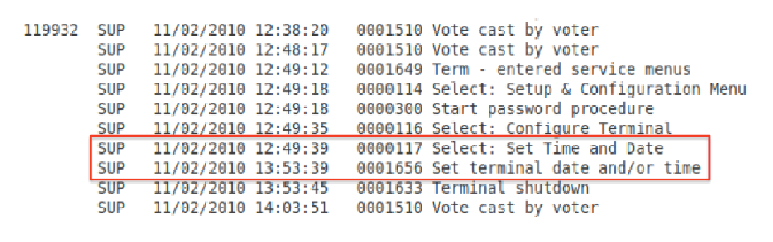
\includegraphics[width=0.5\textwidth,height=0.1\textheight]{ResetClock.eps}
\end{center}
\caption{Event log entry for resetting an iVotronic clock by one hour in Georgetown County.}
\label{fig:one-hour-reset}
\end{figure}

Anomalous time changes were detected in 18 machines. An anomaly is any
occurrence of an unexplained date change while a machine is open for
voting. Figure~\ref{fig:date-anomaly} is an example that occurred in Richland
County. The machine was manually corrected about 30 minutes later.  

\begin{figure}[htbp]
\begin{center}
    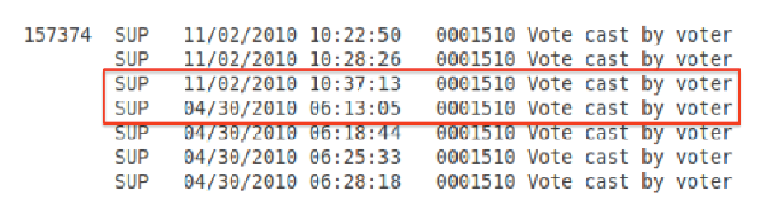
\includegraphics[width=0.5\textwidth,height=0.1\textheight]{DateAnomaly.eps}
\end{center}
\caption{The event log shows a seemingly random date anomaly, which occurred in Richland County during the election day.}
\label{fig:date-anomaly}
\end{figure}

\subsection{Missing Votes}
Our analysis shows that a total of 15 PEBs containing 2082 votes were not
uploaded from the 14 counties that we audited in South
Carolina. Figure~\ref{fig:pebs-not-uploaded} summarizes the PEBs not uploaded
during the General 2010 elections.  

\begin{figure}[htbp]
\begin{center}
    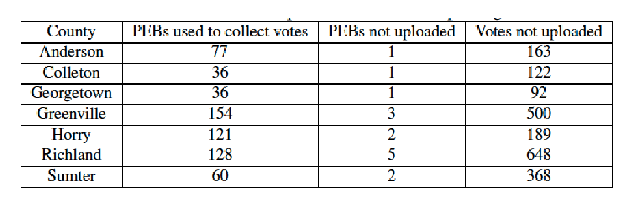
\includegraphics[width=0.5\textwidth,height=0.1\textheight]{PEBsNotUploaded1.eps}
\end{center}
\caption{The number of PEBs and their corresponding votes per county that were not uploaded.}
\label{fig:pebs-not-uploaded}
\end{figure}

AuditBear also identified a few instances of machines not being closed. A
machine must be closed in order to collect the votes and audit data from that
machine. There was a single machine that was not closed in each of the following
counties: Greenville County, Horry County, and Sumter County. None of the races in 
the South Carolina 2010 elections were close enough for 2082 votes to affect the 
outcome~\cite{scResults}. If this 
was a close election, information such as this could be cause for an extensive audit 
or recount of the votes.  

Figure~\ref{fig:greenville-logs} shows some of AuditBear's output on Greenville
County's log files. 

\begin{figure}[htbp]
\begin{center}
    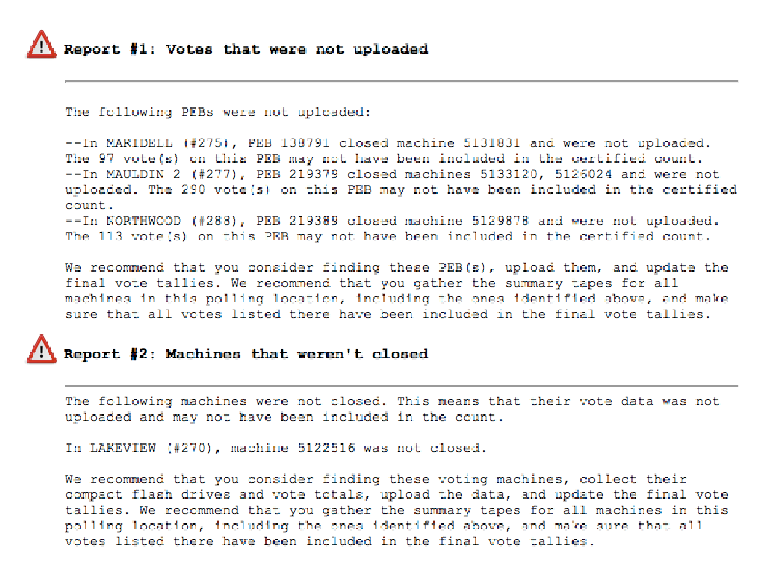
\includegraphics[width=0.5\textwidth,height=0.3\textheight]{VotesNotUploaded.eps}
\end{center}
\caption{Feedback generated by AuditBear for officials when detecting that some votes were not uploaded.}
\label{fig:greenville-logs}
\end{figure}

\subsection{Long Lines}
We found 671 out of a total of 942 South Carolina precincts stayed open
late. Berkeley County had the highest incidence of delayed closing times with
$93\%$ of polling locations closing after 7
P.M\@. Figure~\ref{fig:precincts-closed-late} depicts the precincts 
that closed late in Berkeley County. In the future, resources could be allocated
to those polling locations that stayed open the latest to help move their lines
more quickly. To detect possible lines before 7 P.M., we looked at only the
precincts that were open late. Figure~\ref{fig:long-lines} show the time periods
when the Berkeley County precincts experienced long lines before 7
P.M. Figure~\ref{fig:mann-whitney-u} shows the details of the results of the
Mann Whitney U statistical test for long lines.

\begin{figure}[htbp]
\begin{center}
    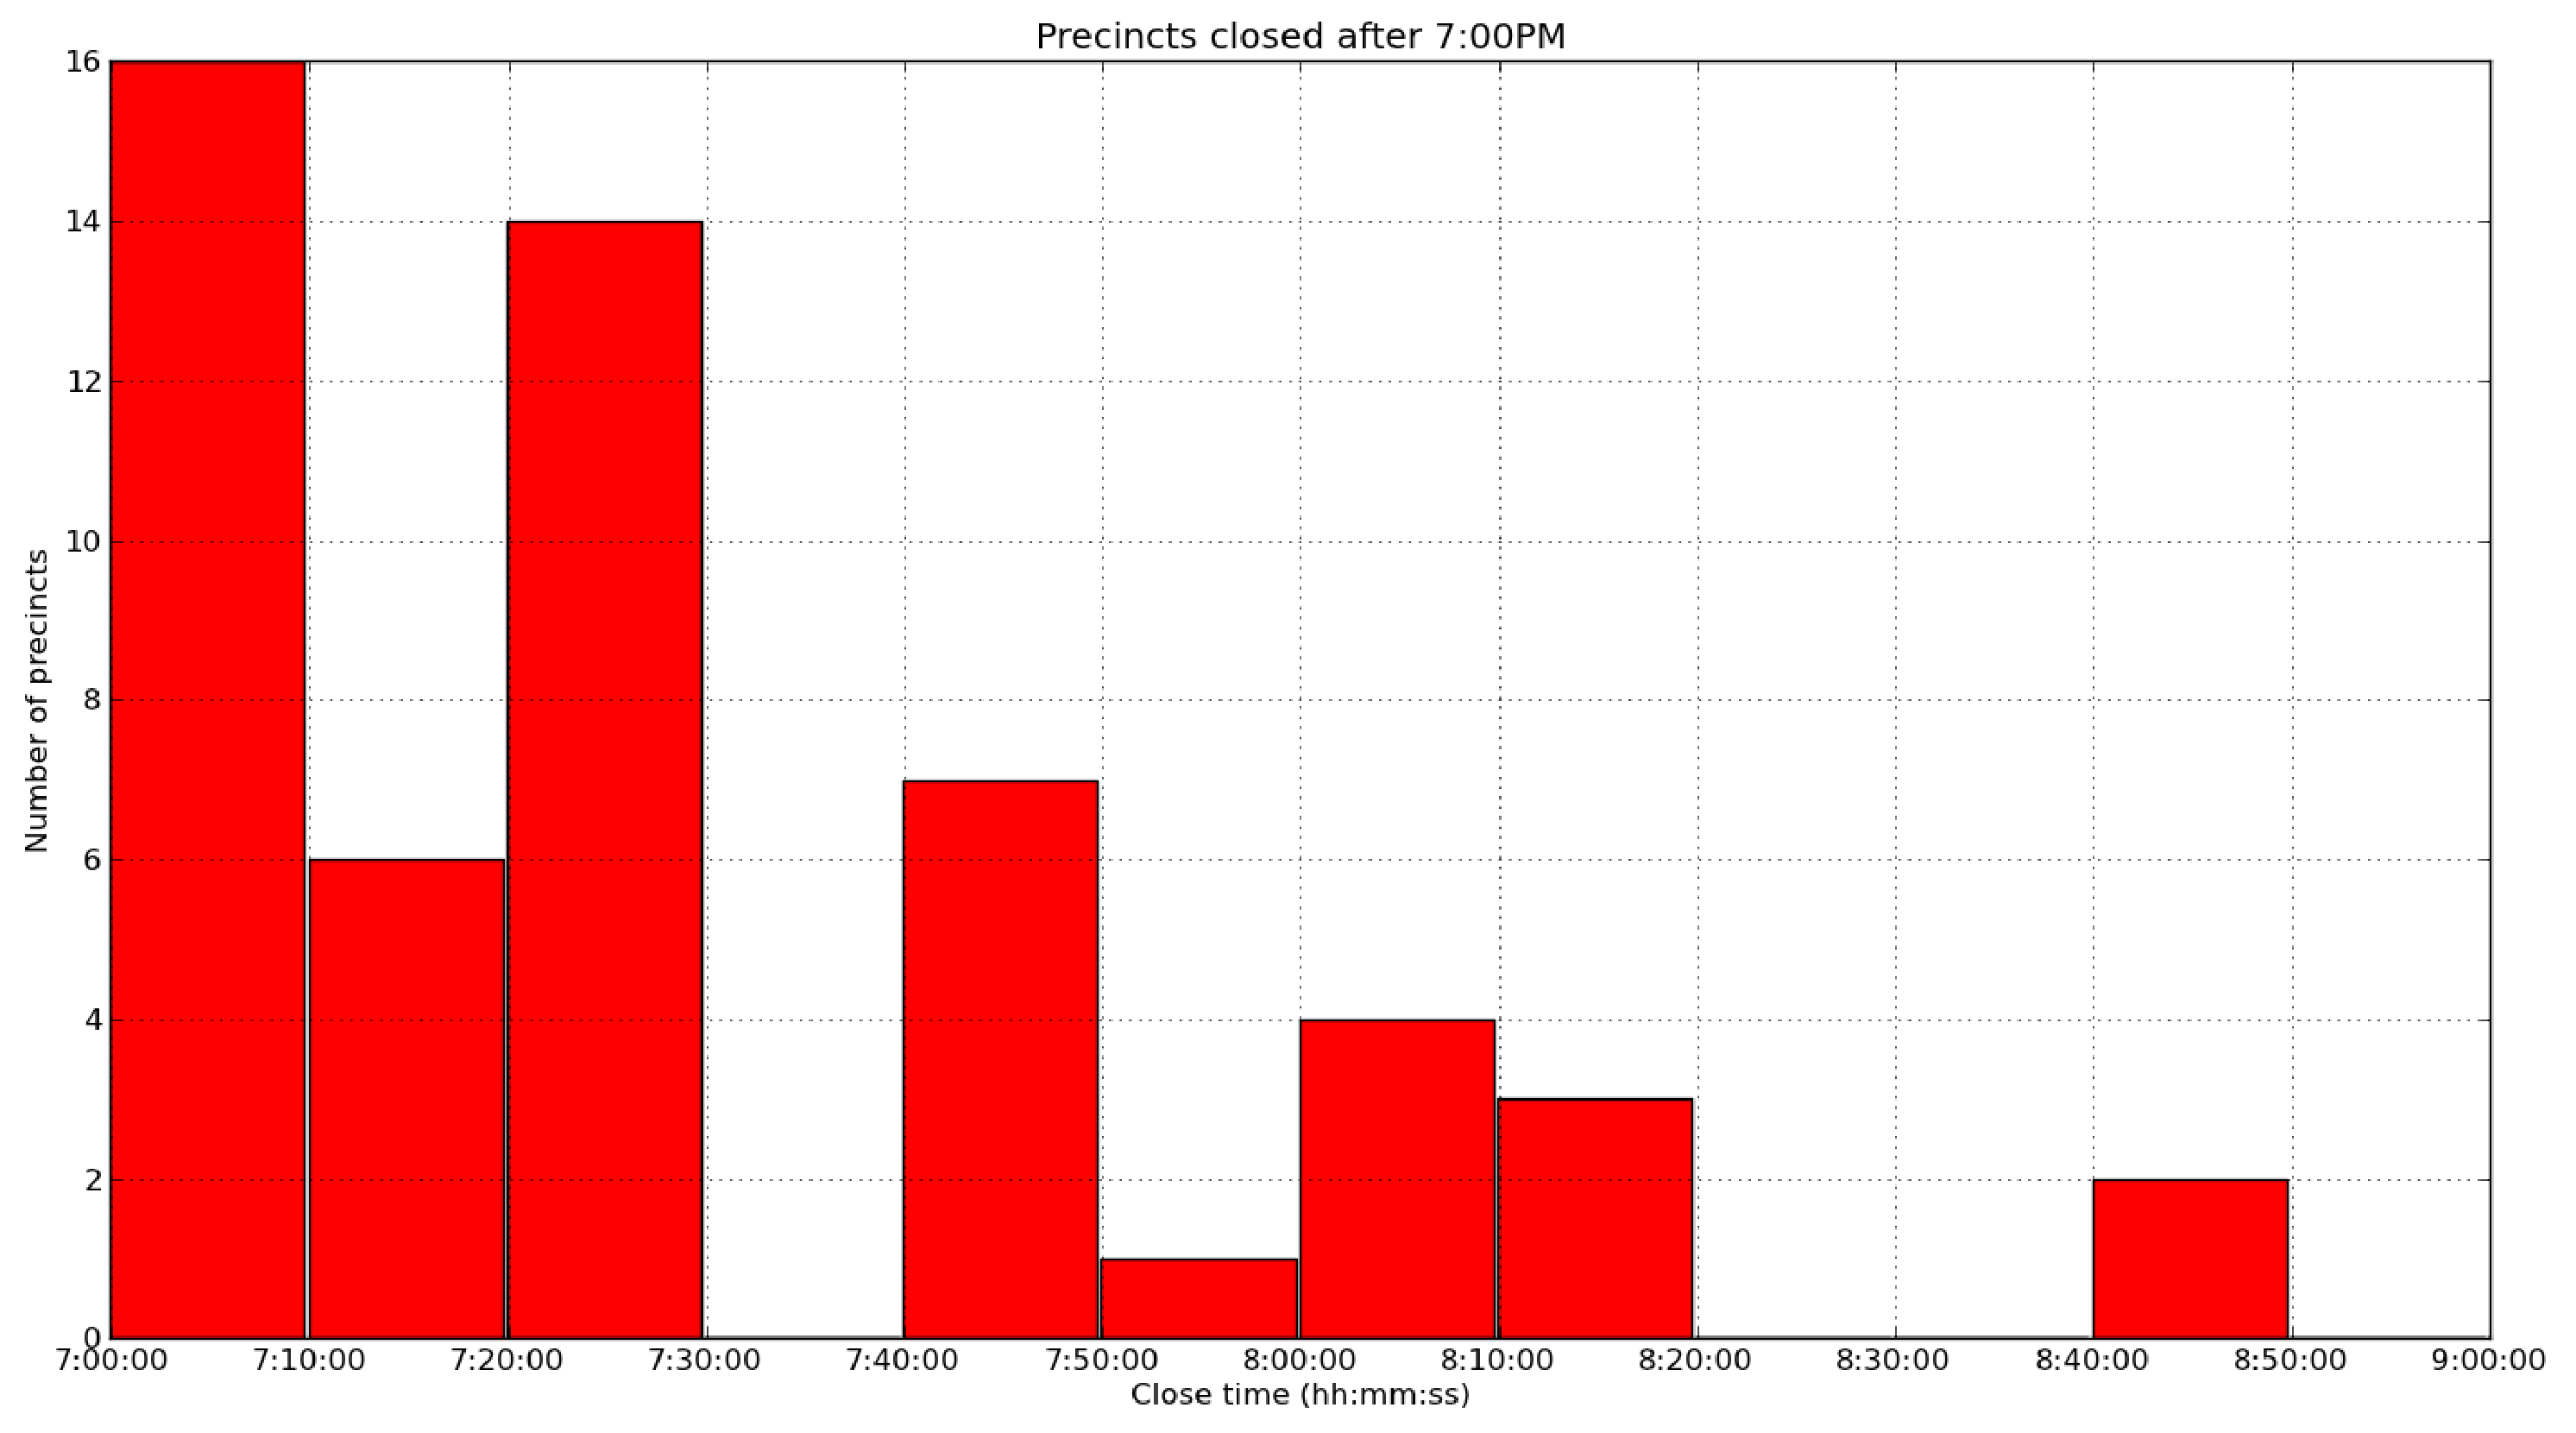
\includegraphics[width=0.5\textwidth,height=0.3\textheight]{berkeleyopenlate.eps}
\end{center}
\caption{The number of precincts that closed within certain time intervals after 7:00 P.M. (late) in Berkeley County.}
\label{fig:precincts-closed-late}
\end{figure}

\begin{figure}[htbp]
\begin{center}
    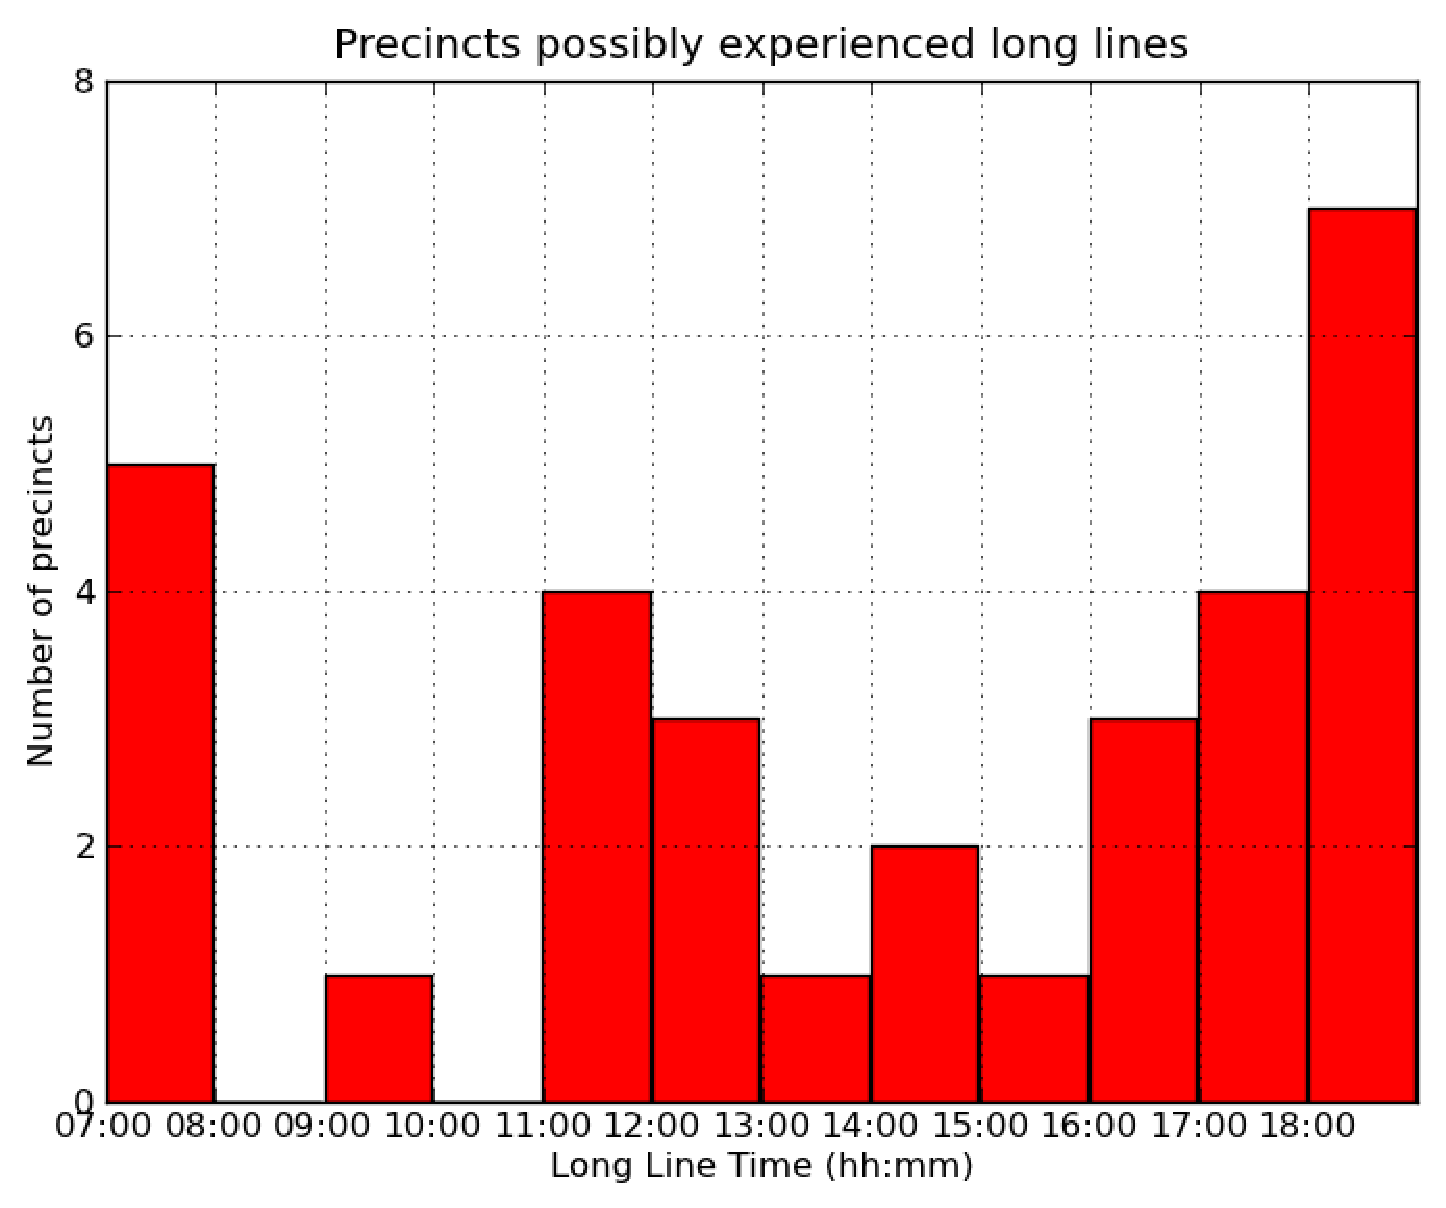
\includegraphics[width=0.5\textwidth,height=0.3\textheight]{berkeleyLongLine.eps}
\end{center}
\caption{The number of precincts that may have experience long lines within certain time intervals in Berkeley County.}
\label{fig:long-lines}
\end{figure}

\begin{figure}[htbp]
\begin{center}
    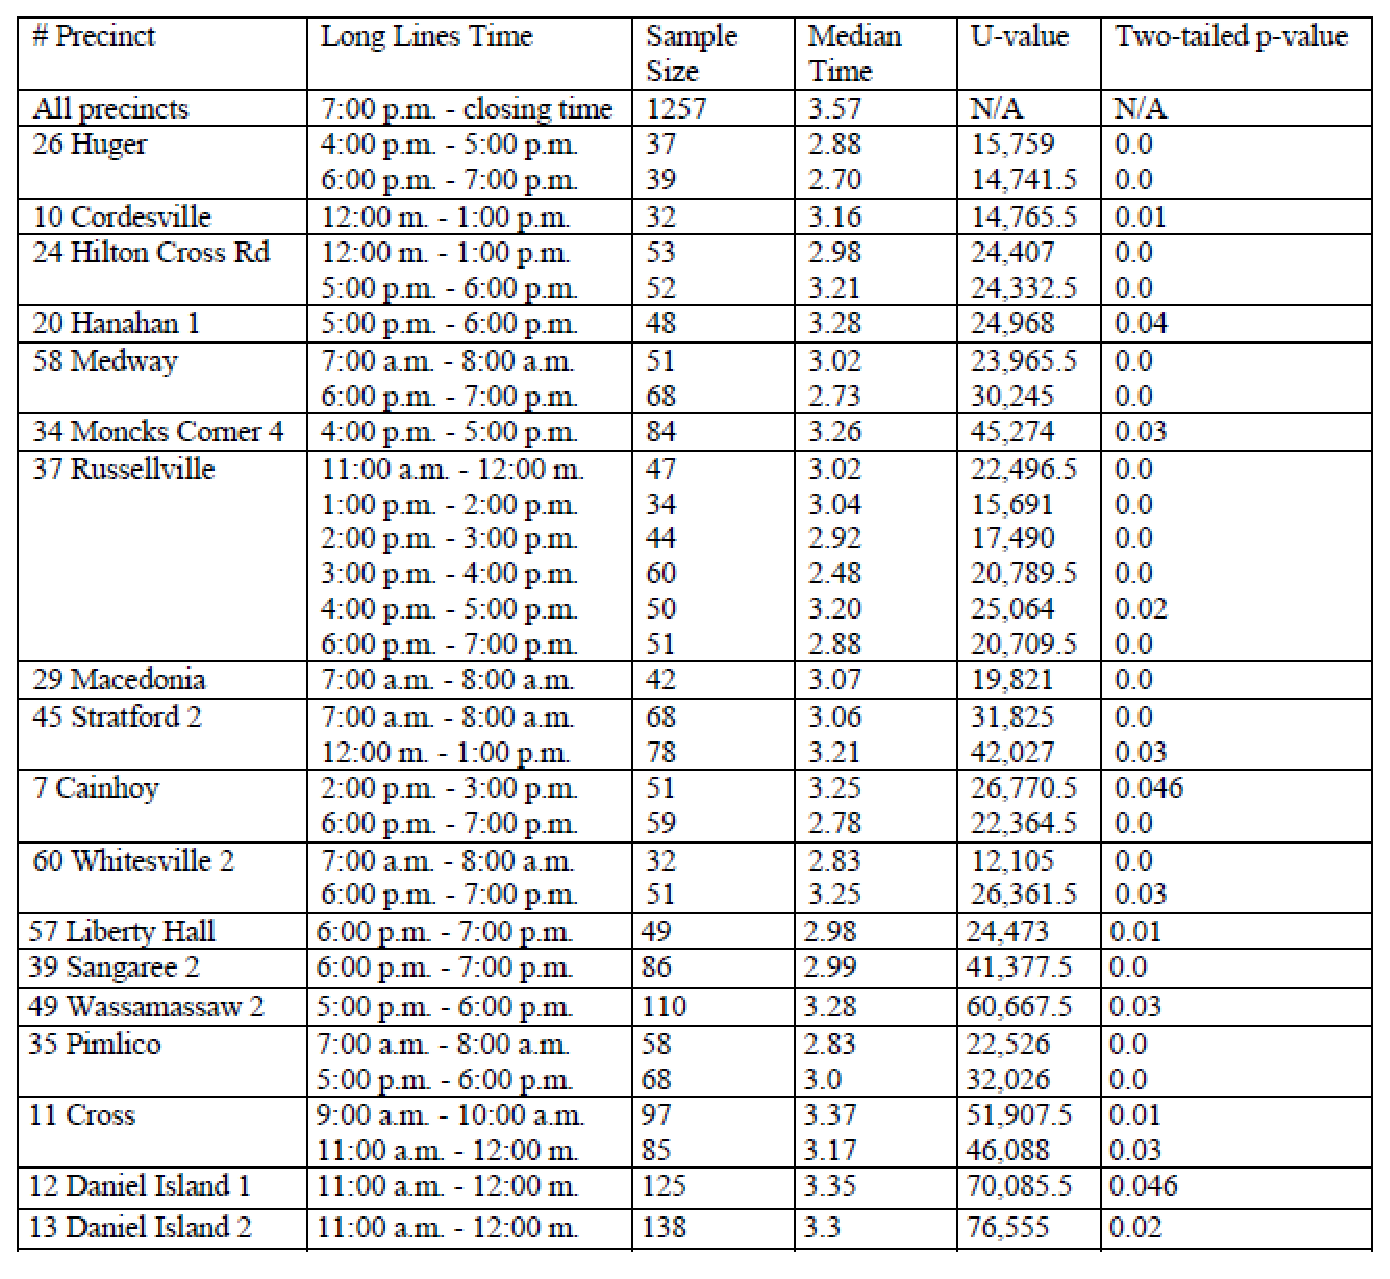
\includegraphics[width=0.5\textwidth,height=0.4\textheight]{berkeleyLongLineTable.eps}
\end{center}
\caption{Times when there were likely long lines in Berkeley County on a per-precinct basis.}
\label{fig:mann-whitney-u}
\end{figure}

\subsection{Calibration Errors}
 We found seven counties where at least one machine was possibly not calibrated
when votes were cast on that machine. An uncalibrated display could potentially
cause votes to not be cast as intended. Our report suggests an election official
or technician inspect these machines for possible calibration issues; see
Figure~\ref{fig:calibration-issues}.


\begin{figure}[htbp]
\begin{center}
    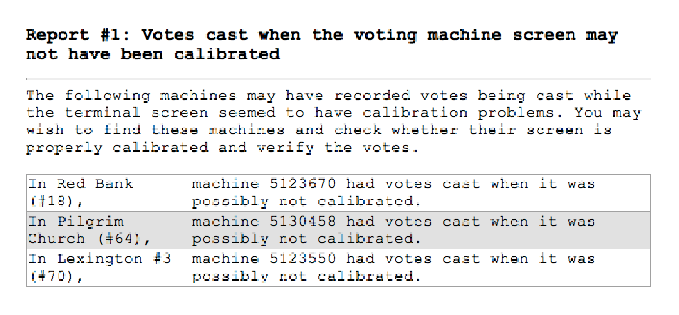
\includegraphics[width=0.5\textwidth,height=0.2\textheight]{NotCalibrated.eps}
\end{center}
\caption{Feedback generated by AuditBear for election officials when calibration issues are detected.}
\label{fig:calibration-issues}
\end{figure}

\subsection{Procedural Errors}
Our findings reveal the need for improvements in poll worker training. When
opening and closing a machine, the same master PEB should be used, but in 11
counties there were machines opened and closed with different PEBs. Our results
showed an association between this error and certain precincts where poll workers
made those mistakes repeatedly. \comment{The event of opening and closing a machine 
usually happens only once or twice on each machine in a precinct; therefore, 
when this error occurs, it creates a high error percentage for the precinct.} 
When this error is made multiple times at a single precinct, it indicates 
that perhaps the poll workers do
not know the procedures, whereas a random distribution of these errors across
polling locations probably means a mistake was made. Colleton County had five
instances of this procedural error, but four of those instances took place at
one polling location. Figure~\ref{fig:diff-pebs-open-close} shows this report
from Colleton County.  

A poll worker assigns each voter a PEB to use when it is that voter's turn. When 
voters cast votes, they should not do so with a Master PEB. For most precincts
in Florence County, this error never occurred, however, four precincts had large
numbers of this error; Mill Branch had  
this error on 56 out of 540 votes, Pamplico 2 had this error on 82 out of 579 
votes, McAllister Hill had this error on 102 out of 749 votes, and Effingham 
had this error on 86 out of 591 votes. This pattern of errors again suggests
certain poll workers did not know the proper
procedure. Figure~\ref{fig:master-peb-activated}  
shows this relationship in Florence County. 

\begin{figure}[htbp]
\begin{center}
    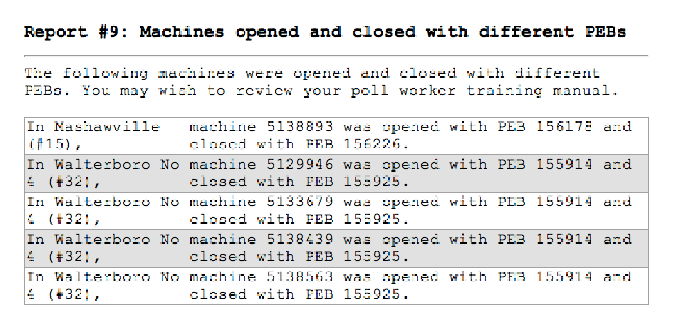
\includegraphics[width=0.5\textwidth,height=0.2\textheight]{OpenClosePEBs.eps}
\end{center}
\caption{An example response when AuditBear reports machines that were opened and closed with different PEBs.}
\label{fig:diff-pebs-open-close}
\end{figure}

\begin{figure}[htbp]
\begin{center}
    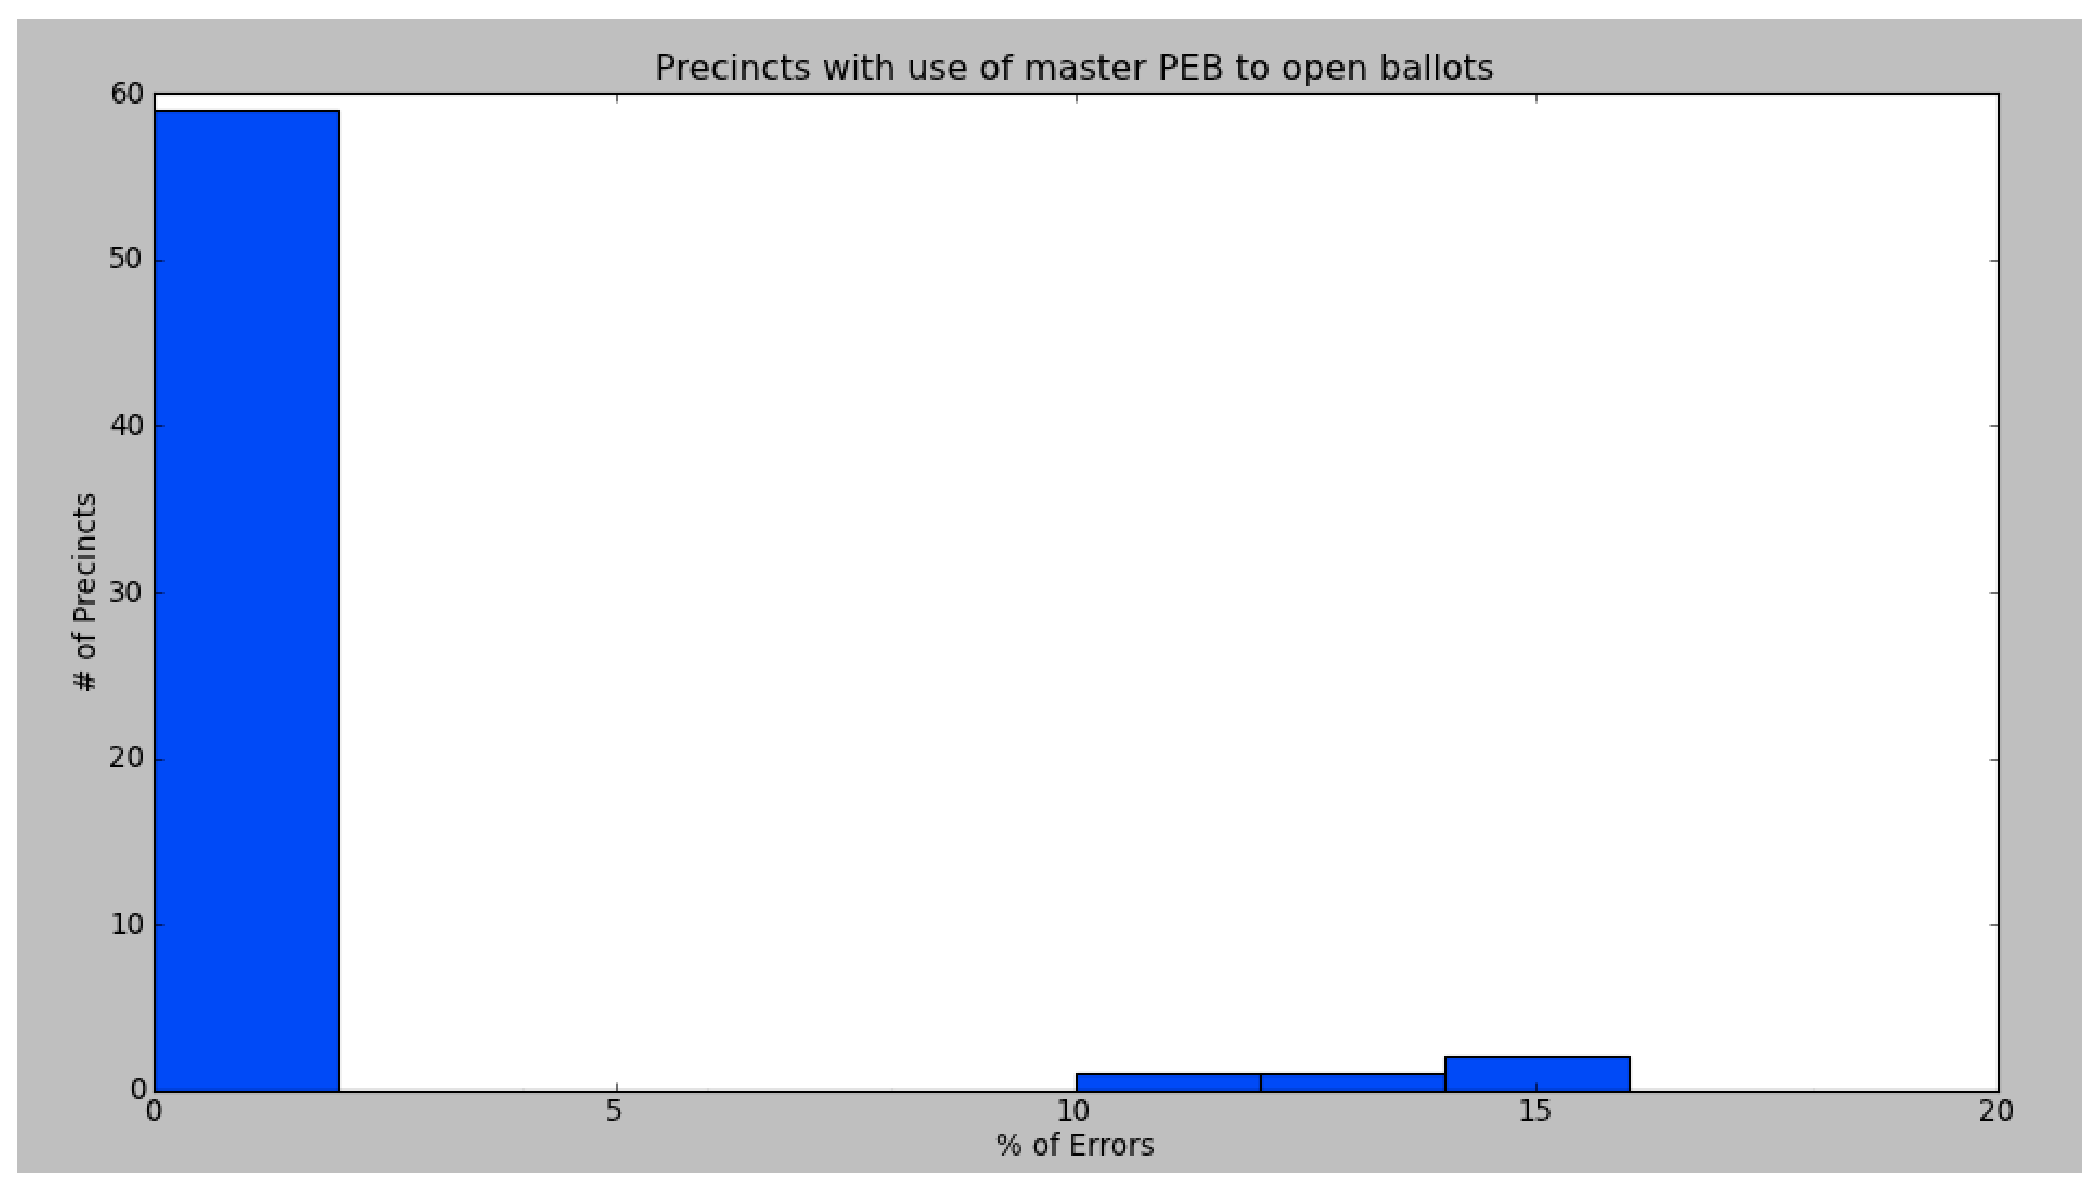
\includegraphics[width=0.5\textwidth,height=0.4\textheight]{PEBactivateHist.eps}
\end{center}
\caption{This histogram shows the percentage of votes at each precinct that were 
cast with a Master PEB.  The precincts that showed the highest percentages had 
between 56 and 102 instances of this error.}
\label{fig:master-peb-activated}
\end{figure}

\subsection{Audit Data}
 In several counties, the audit logs appeared to be incomplete. Our analysis
 detected six counties that did not have the same set of machines in both the
 event log and ballot images file. Florence County had the most inconsistencies
 with 65 machines that had votes cast on them according to the event log, but no
 ballot images. We also saw cases where there were ballot images for votes cast
 on machines that did not record any events on the event log. In addition to an
 unusually large amount of missing data, the analysis of Florence County showed
 machines that did not have the same number of votes cast as ballot images. See
 Figure~\ref{fig:incomplete-audit-data} for example output from AuditBear. 

\begin{figure}[htbp]
\begin{center}
    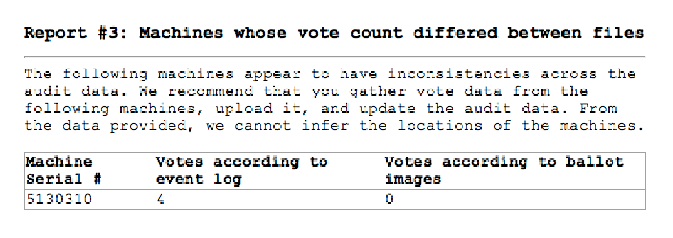
\includegraphics[width=0.5\textwidth,height=0.2\textheight]{IncompleteAuditData.eps}
\end{center}
\caption{Feedback generated by AuditBear when incomplete audit data is detected.}
\label{fig:incomplete-audit-data}
\end{figure}

\section{Future Voting Systems Suggestions}
\label{sec:suggestions}
We believe the following recommendations will make audit files more usable. 

Voting systems should support automatic generation and collection of audit logs 
in a central location. \comment{Not many systems have this capability, which is essential 
for third-party analysis.} While many other DRE systems do capture data in their audit logs similar to what
the iVotronic does, no other widely deployed voting system makes it as easy to
gather all the audit logs from all of the voting machines into a single
place. As a result, while our methods are in principle applicable to other
deployed voting systems, in practice this would require additional effort from
election officials. 
 In addition, audit logs should have a universal 
electronic file format.  This would allow for a more extendable tool.

Future voting system standards introduce stronger
requirements for audit logs; this could make it easier to apply our analyses to
other voting systems~\cite{Wagner2010}. \cks{What exactly are those stronger
  requirements? Are they the same as what we're suggesting here? A subset?
  Superset? Depending on the answer, this piece might do better at the end of
  the section.} 

Vendors should document the meaning of all events. We found audit logs with
event messages, such as ``UNKNOWN,'' ``Warning – PEB I/O flag set,'' and
``Warning – I/O flagged PEB will be used,'' which sound ominous, however we
could not determine the gravity of the issue. Despite combing through all of
ES\&S’s publicly available information about the iVotronic, the meaning of these
events still remain a mystery~\cite{VerVot2011, ESS2011a, ESS2011b}. 
 
Accuracy of date and time logging needs improvement. When the machine has an
incorrect clock, timestamps are inaccurate and it becomes difficult to recreate
election day events. In addition, some audit log analyses, such as the open late
analysis, are made more difficult by unreliable timestamps. 
 
Make system manuals available to the public. Voting machine audit logs are
public information. The general public can request them under the Freedom of
Information Act. In the same fashion, we recommend that voting system manuals be
made freely available. This would allow the public to see for themselves if
there were any problems that should be addressed.  
 
Capture the ballot activation event. Recording the time each ballot is activated
(as opposed to only recording when the ballot is cast) would make it easier to
learn when the voting machines were heavily used and when they were idle. As the 
ballot images file is still randomized, there is still no way to connect a voter 
to his or her vote.  Even if a spectator watches the polling location and records 
how long each voter spends in the voting booth, there are hundreds (if not thousands) 
of ballot images in the ballot images file.  It is unlikely that a malicious person 
could use this information in order to determine a voter's choice.  This
is a simple change that would not compromise voter privacy, and would make it
simple for an automated tool such as AuditBear to extract information
about long lines during the day.
 
 \section{Related Work}
Two recent studies used event logs from the iVotronic voting system to audit
elections~\cite{Buell2011, Sandler2007}. Buell et al.~\cite{Buell2011} analyzed
the same South Carolina elections that we did and also discovered votes not
included in the certified counts and problems with the audit data. By consulting
additional audit materials, such as the printed results tapes, the authors were
able to offer possible explanations for why the problems occurred. Our work
takes a slightly different approach. We focus on developing an automated
analysis of the publicly available audit log data that can be used by
anyone to detect other possible errors in addition to missing votes. \comment{While our tool 
did discover and report similar problems, we simply
report what was wrong, but can not provide a possible explanation for the cause
of the error as we do not have access to printed results tapes.}  

Sandler et al.~\cite{Sandler2007} analyzed vote tallies by comparing each
machine's protected vote count to the printed results tapes. Their report also
finds time-stamps that were most likely inaccurate. With further investigation,
they concluded that the machine hardware clock was incorrect. Our research
provides analyses to identify similar problems, but in a way that can be
automated.   

There has also been research on using the audit logs to analyze election-day
procedure and activity. Antonyan et al. showed how event logs could be used to
determine if a machine acted ``normally'' on election
day~\cite{Antonyan2009}. They built a finite state machine that models the
sequences of events that a well-behaved AccuVote-OS scanner might produce and
used it to analyze AccuVote-OS logs. This type of analysis could be useful for
the iVotronic systems that we studied, too.  

Other work has focused specifically on detecting or predicting long
lines. Formal models adapted from queuing theory and simulations of voter queues
can be used to better understand the factors that affect the length and duration
of lines at the polling place~\cite{Allen2006, Edel2010}. Our work is
complementary, and in fact information about election day events gathered by
AuditBear can be used to inform the queuing models. A field study, such as that
done by Spencer and Markovitz~\cite{Spencer2010}, can provide ground truth about
the occurrence of long lines on election day, but in the absence of that ideal,
our analysis can provide some information about the time and duration of long
lines. 

Voter Verified Paper Audit Trails (VVPATs) are a different type of audit
log. Unlike the audit logs we used in our analyses, VVPATs are viewed and
verified by the voter and are more suited to audits concerning a DRE incorrectly
capturing a voter’s intent. Our work is more concerned with identifying cases of
cast votes not being included in the final count, or issues at the polling place
that might prevent the voter from casting their vote in the first place. With
VVPATs, as long as a certain percentage of voters do check their paper
ballot~\cite{Hall2006}, the voting machine need not be assumed correct, whereas
our analyses do make this assumption. 

\section{Conclusion}
This paper develops methods to analyze audit data from DRE voting machines. It 
introduces new methods for extracting information about election-day activities
and post-election anomalies from audit data.\comment{; these include 
possible miscounts, procedural errors, voting machine malfunctions, and system 
deficiencies. In addition, we present a new way to detect long lines and }  
We conduct an audit on the 2010 South Carolina 
election using these methods and are able to detect instances of missing votes,
procedural errors, and likely instances of lines throughout the day. With this
information, election officials can improve poll worker 
training, resource allocation, election tabulation procedures, and 
voting machine preparation testing. Based on our experience during this
research, we make suggestions for future audit logs that would make an automated
analysis such as ours even more informative.
 
We built a web application, AuditBear, to perform these analyses. Users can
upload the iVotronic log files to our website and run the analyses. By automating our
analyses we can provide intelligent feedback to election officials during the
canvassing process and help them quickly correct any problems in order to
produce accurate election results. AuditBear is freely available online.  
 

%\section{Acknowledgments}
%Leave out for anonymization.

{\footnotesize \bibliographystyle{acm}
\bibliography{../Latex/paper2.bib}}

%Appendix
\clearpage
\onecolumn
\begin{center}
\appendix
\section{Event Log File}\label{app:el} 
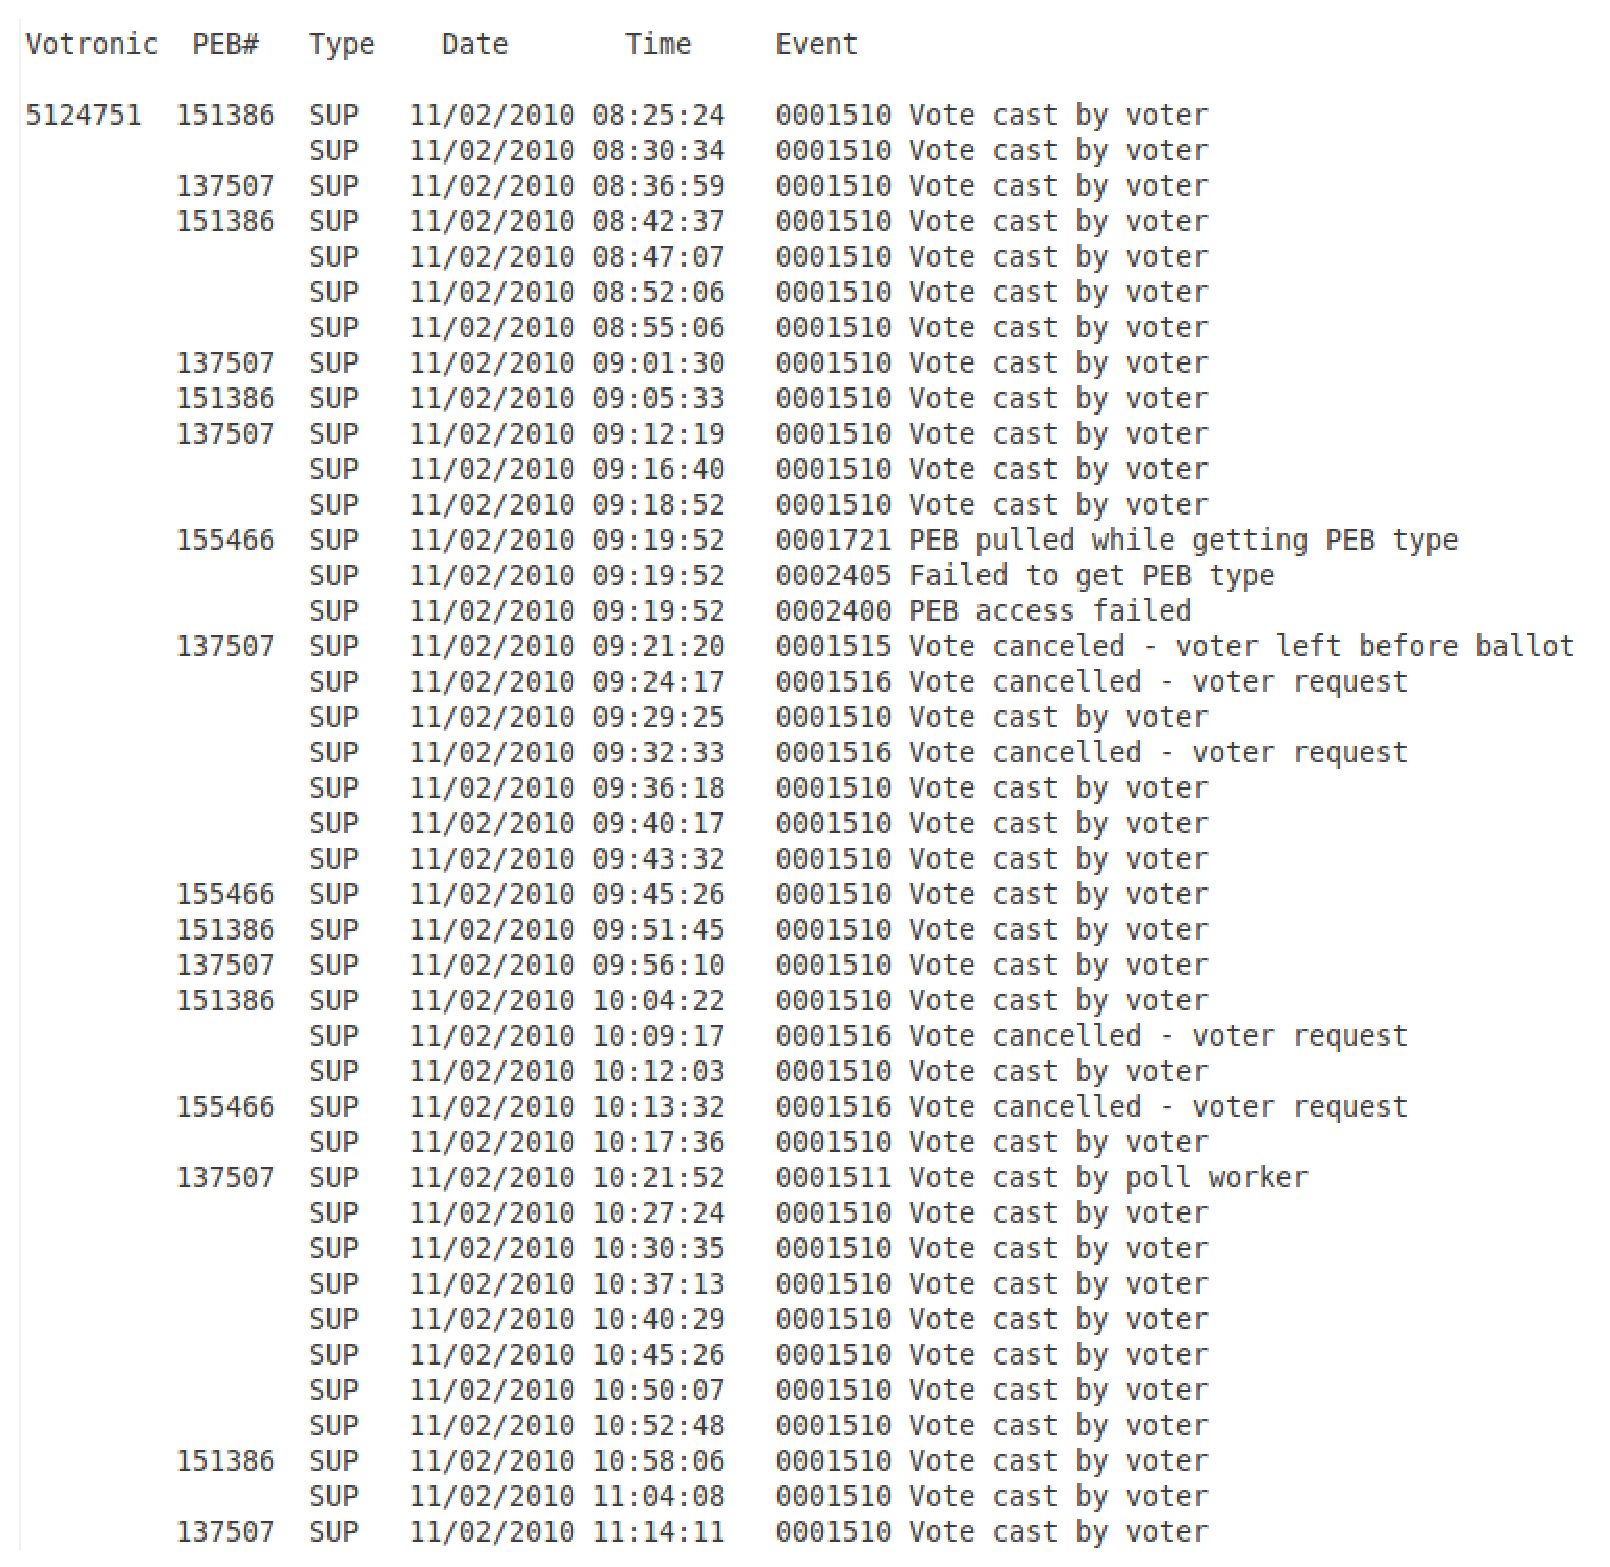
\includegraphics[width=0.8\textwidth]{eventLog.eps}
%~\ref{app:el}

\clearpage
\section{Ballot Image File}\label{app:bi}
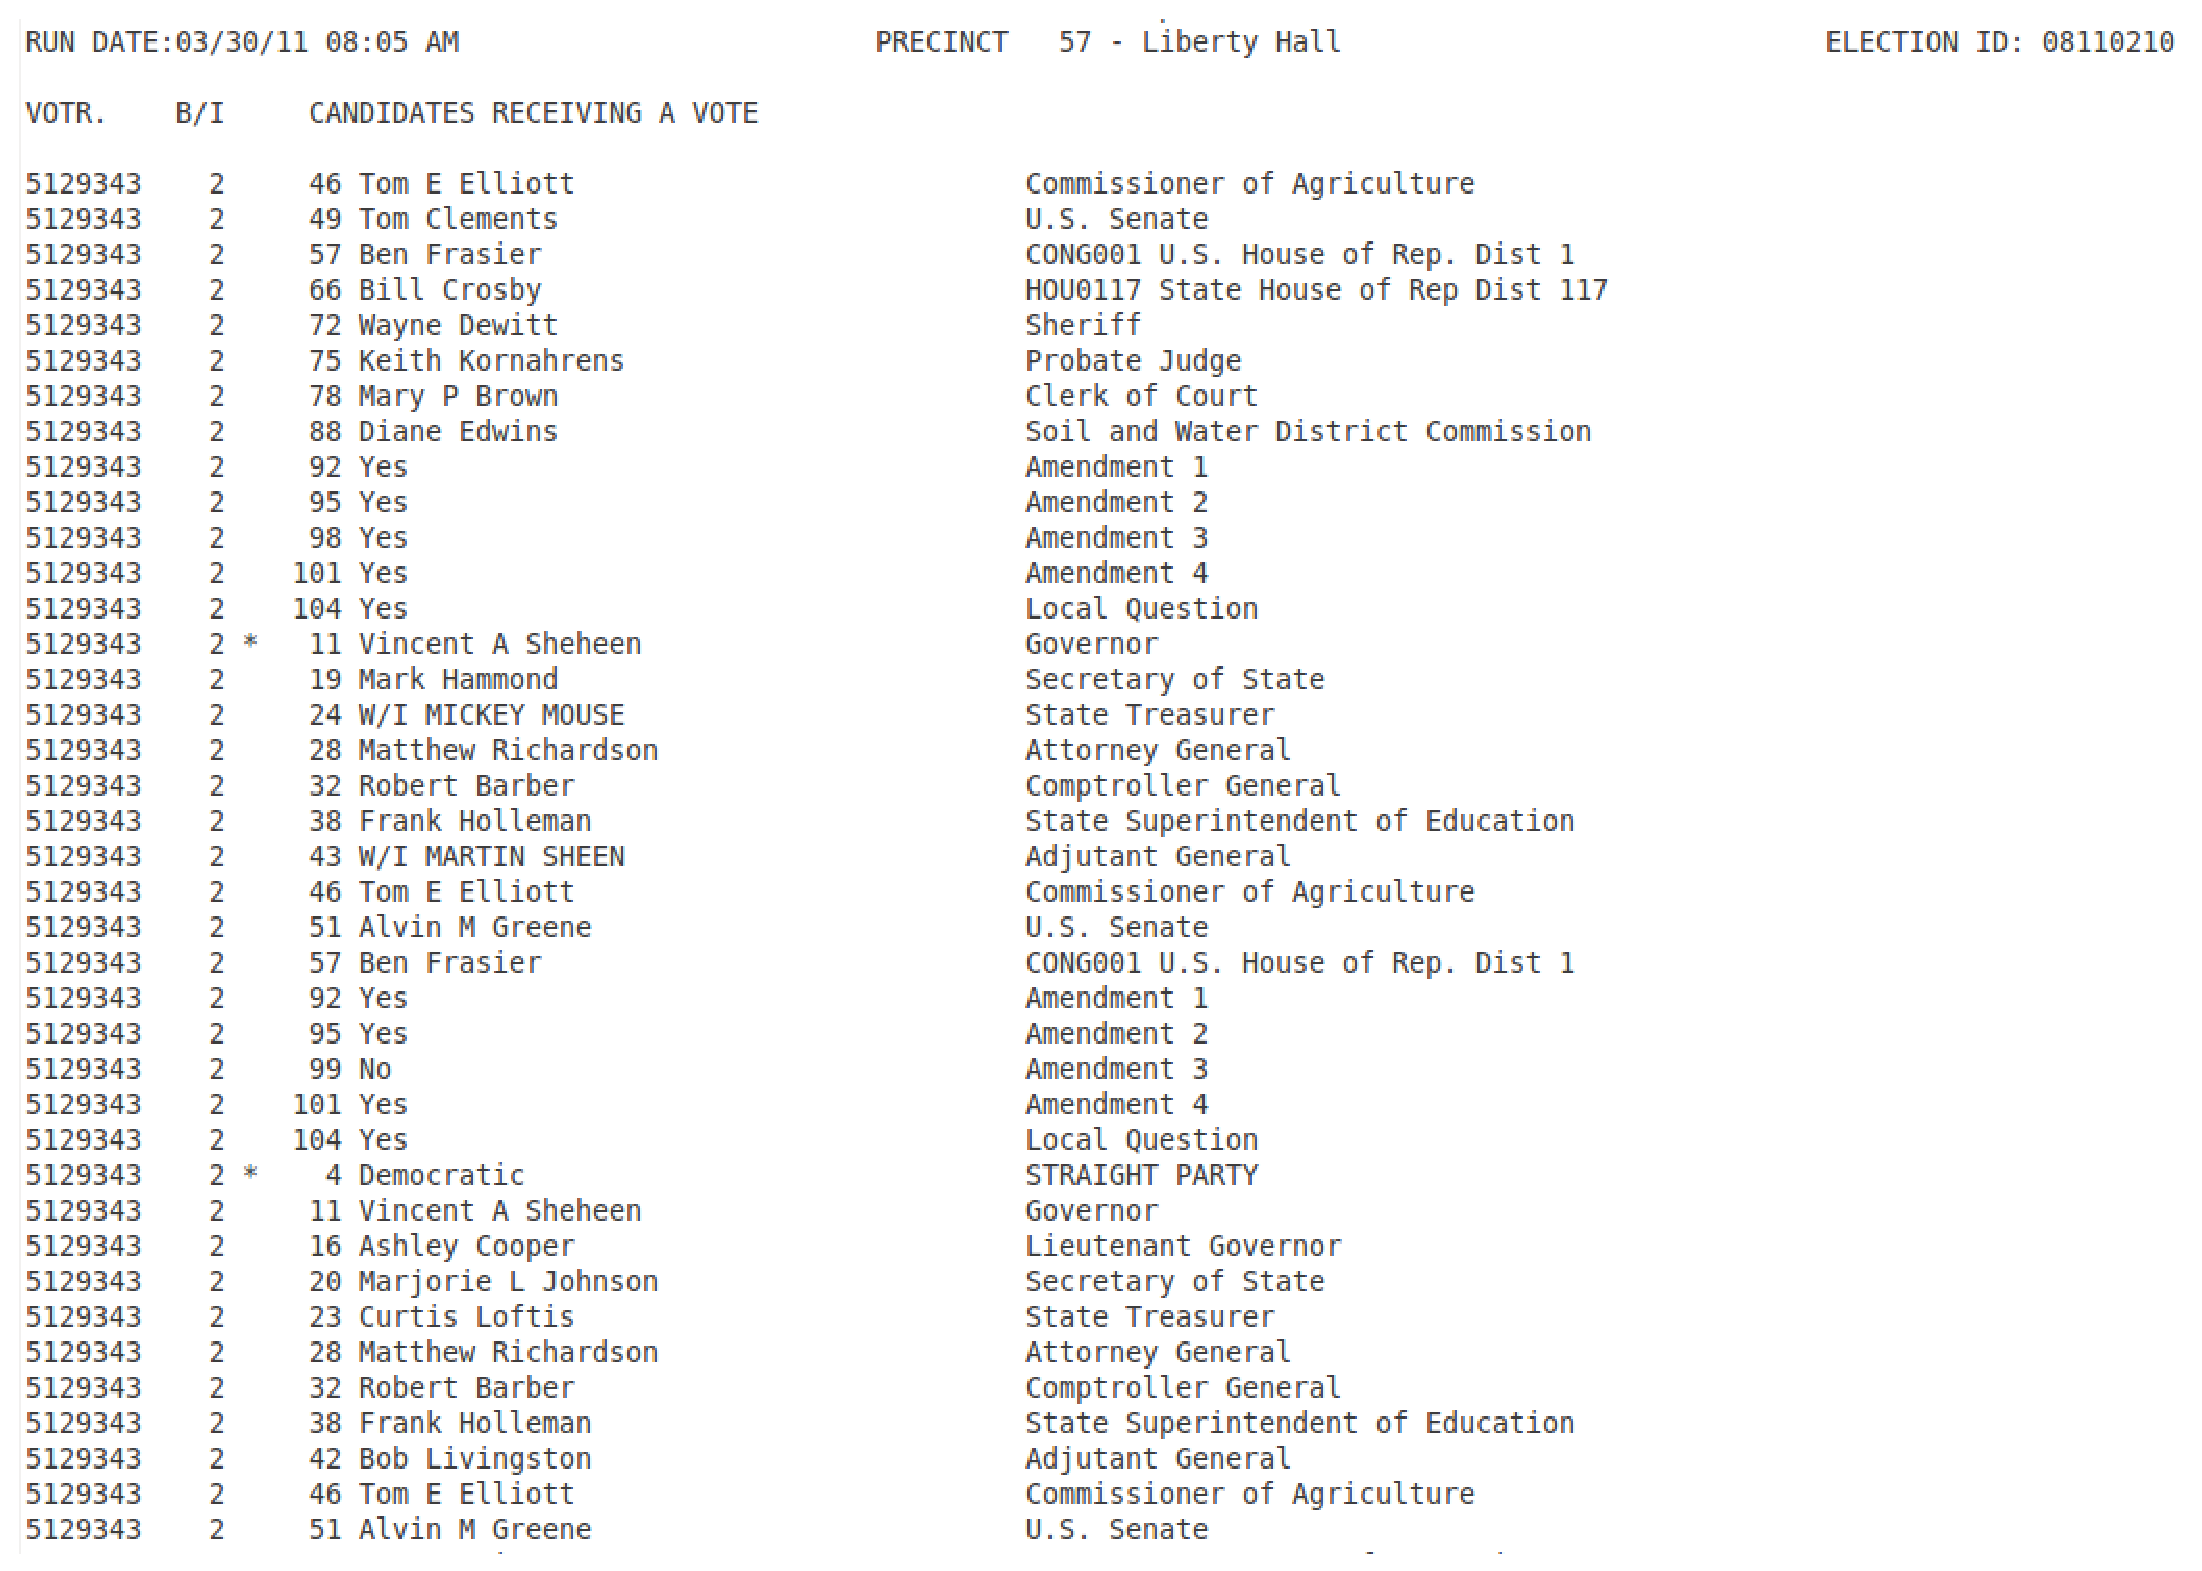
\includegraphics[width=0.9\textwidth]{ballot.eps}
%This is app~\ref{app:bi}

\clearpage
\section{System Log File}\label{app:sl}
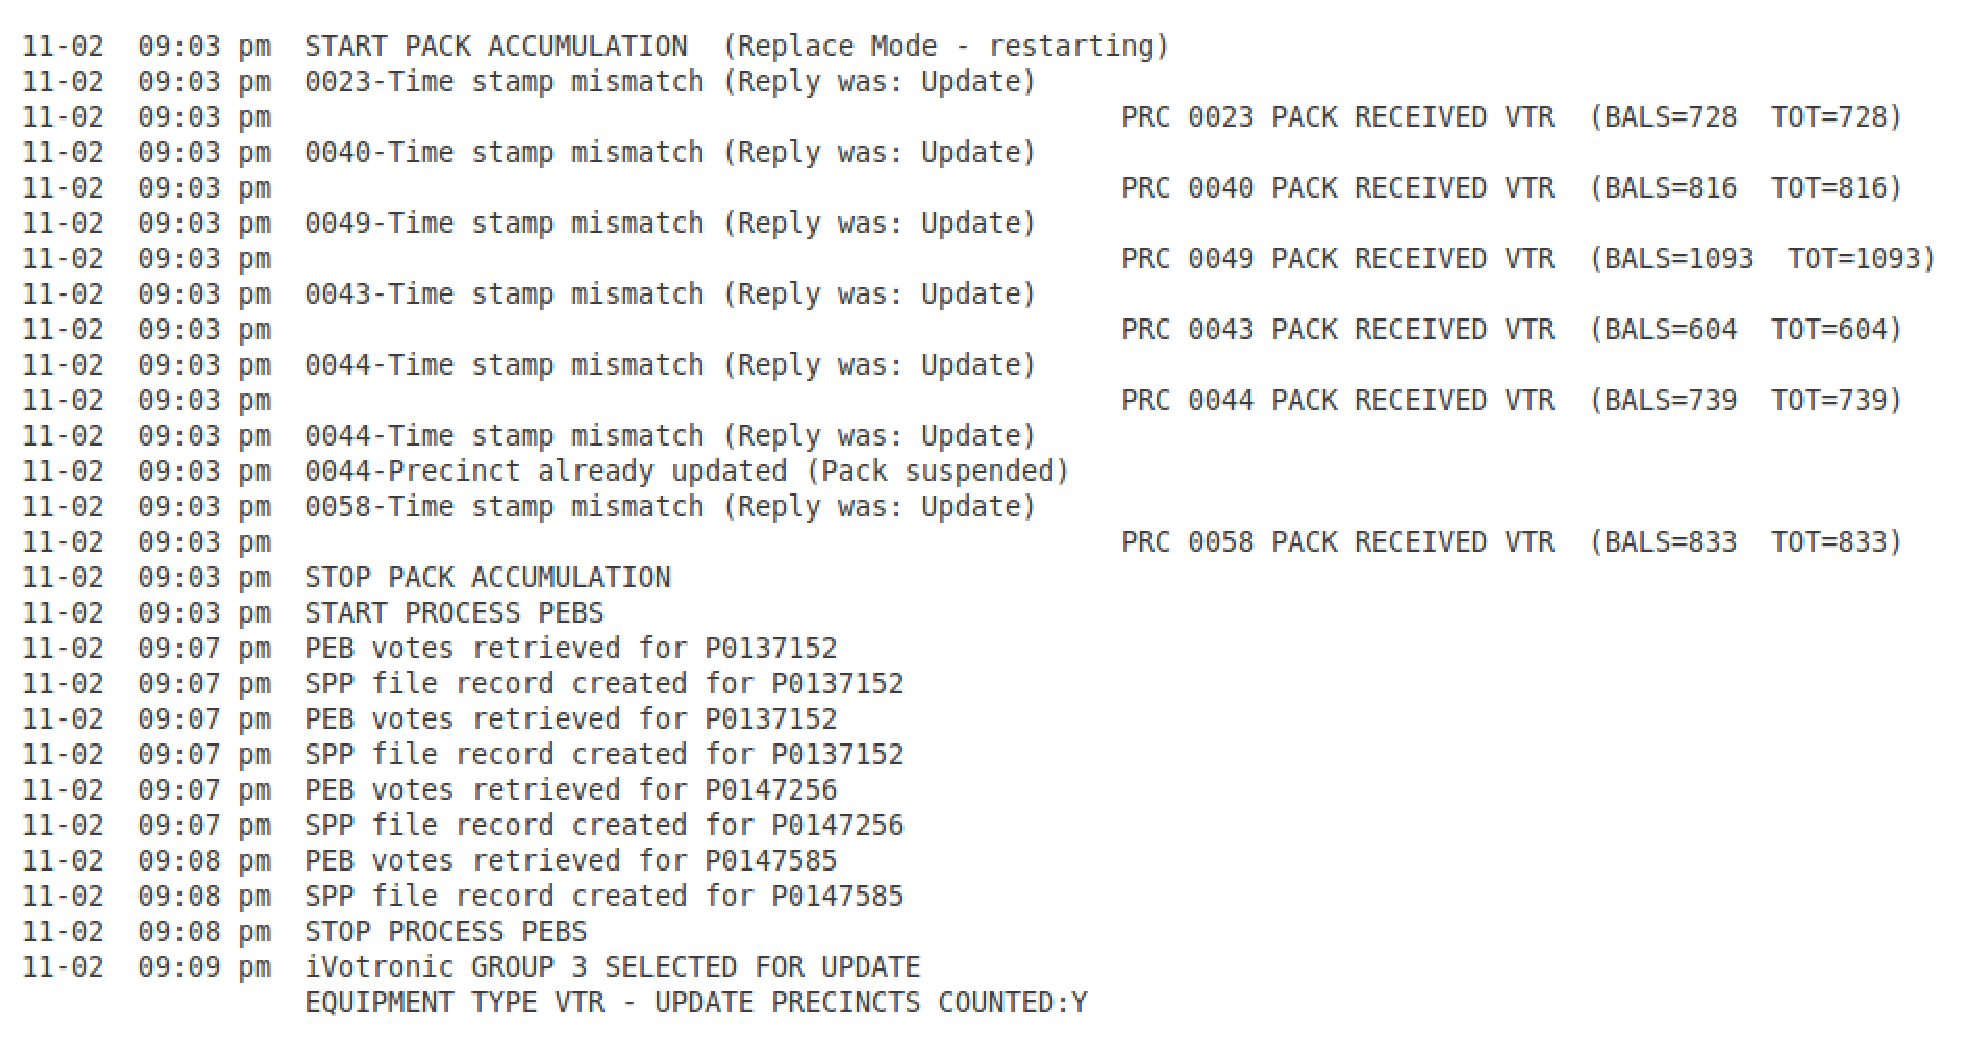
\includegraphics[width=0.9\textwidth]{system.eps}
%This is app~\ref{app:sl}
\end{center}

%\theendnotes

\end{document}







